\documentclass{beamer}
\usepackage[utf8]{inputenc}
\usepackage{fontenc}
\usepackage{bm}
\usepackage{ragged2e}
\usepackage{graphicx}
\usepackage{amsmath}
\usepackage{gensymb}
\usepackage{csquotes}[british]
\usepackage{natbib}
\bibliographystyle{plainnat}

\usepackage{styles/beamerthemePOLIbeamer}

\apptocmd{\frame}{}{\justifying}{} % Allow optional arguments after frame.

\graphicspath{{./styles/img/figs/}}

\setcounter{MaxMatrixCols}{20}

\DeclareMathOperator{\atantwo}{atan2}

% Title Page
\title{EKF-SLAM for drone localization}
\subtitle{Thesis project - Leonardo Drone Contest}
\date{2020}
\author{Diego Emanuel Avila}
\supervisortext{Supervisor:}
\supervisor{Prof. Matteo Matteucci}

% ----------------------------------
\begin{document}

    % ----------------------------------
    %    Title Page
    \begin{frame}
        \pagenumbering{gobble} % < ------------------- PUT THIS!!
        \titlepage
    \end{frame}


    % ----------------------------------
    %    Overview
    \begin{frame}
        \pagenumbering{arabic} % <----------------------  REMEMBER THIS!!!!!!!
        \tableofcontents
    \end{frame}

    %--------------------------------
    \section{Problem}
    \begin{frame}
        \justifying
        \frametitle{Problem}
        In the context of Leonardo Drone Competition, a fully autonomous drone should, in the first round, take off from the base position and inspect the environment in order to generate a map; during the second round, the drone should follow and land on a (previously set) sequence of points. \\[10pt]

        The environment is composed by a set of obstacles of different sizes, 6 landmarks and 10 path-markers, plus the  base marker. \\[10pt]

        The drone should be able to fly and simultaneously map and localize itself in the environment, and be able to identify, store and localize the path-markers, so to follow the predefined path.

    \end{frame}

    % -------------
    \section{Proposed solution}
    \begin{frame}

        \justifying
        \frametitle{Proposed solution}

        Since the drone has not been built yet, I am assuming the information provided by the flight controller will be: %% revisar esto, no es flight controller
        \begin{itemize}
            \item{Drone angular and linear velocities in the global reference frame}
            \item{Poles range and bearing with respect to the local reference frame.}
            \item{Marker pose with respect to the local reference frame (x, y, z, $\phi$, $\theta$, $\psi$)}
        \end{itemize}

        Given this information, the proposed solution involves the development of an EKF-SLAM algorithm, \textit{able to dynamically add markers in the state vector}.

    \end{frame}

    % -------------
    \section{Extended Kalman Filter}
    \begin{frame}
        \justifying
        \frametitle{Extended Kalman Filter}

        The state vector $\bm{\mu}$ in this particular case will be \\ $\begin{bmatrix} \bm{r} & \psi & ... & \bm{m_1} & \bm{m_2} & ... \end{bmatrix}$, where:
        \begin{itemize}
            \item{$\bm{r}$ is the position of the robot in the world reference frame $\begin{bmatrix}x & y & z\end{bmatrix}$}
            \item{$\psi$ is the drone yaw in the world reference frame}
            \item{$\bm{m_i}$ is the pose of the marker i $\begin{bmatrix}x & y & z & \phi & \theta & \psi \end{bmatrix}$}
        \end{itemize}

    \end{frame}

    \begin{frame}
        \justifying

        As known, the Kalman Filter can be divided in 2 steps: \textbf{prediction} and \textbf{correction}:

        \begin{enumerate}
            \item{prediction}
            \begin{enumerate}
                \item{$\hat\mu = g \left( u_t , \mu_{t}  \right) $}
                \item{$\hat\Sigma = G_t \Sigma_{t-1} G_t^T + R_t $}
            \end{enumerate}
            \item{correction}
            \begin{enumerate}
                \item{$K_t = \hat\Sigma H_t^T \left( H_t \hat\Sigma H_t^T + Q_t \right)^{-1}$}
                \item{$\mu_{t+1} = \hat\mu + K_t \left( z_t - h \left( \hat\mu \right) \right) $}
                \item{$\Sigma_{t+1} = \left( I - K_t H_t \right) \hat\Sigma$}
            \end{enumerate}
        \end{enumerate}

    \end{frame}

    \begin{frame}
        \justifying

        \begin{columns}
            \begin{column}{0.68\textwidth}
                \begin{itemize}
                    \item{g$\left( \boldsymbol{\cdot} \right)$ is the vehicle kinematics or motion model, which involves the motion noise, the control variables $\bm{u}$ at time t and the state vector $\bm{\mu}$ in the previous time step.}
                    \item{$G_t$ is the Jacobian matrix of the motion model g, $\Sigma$ the covariance matrix in the previous time step and R, which provides a mapping between the motion noise in control space to the motion noise in state space}
                \end{itemize}
            \end{column}
            \begin{column}{0.32\textwidth}
                \begin{align*}
                \color{slidesRed} \hat{\mu}  & \color{slidesRed}= g \left( u_t , \mu_{t}  \right)                \\
                \color{slidesRed} \hat\Sigma & \color{slidesRed}= G_t \Sigma_{t-1} G_t^T + R_t                   \\
                K_t                          & = \hat\Sigma H_t^T \left( H_t \hat\Sigma H_t^T + Q_t \right)^{-1} \\
                \mu_{t+1}                    & = \hat\mu + K_t \left( z_t - h \left( \hat\mu \right) \right)     \\
                \Sigma_{t+1}                 & = \left( I - K_t H_t \right) \hat\Sigma
                \end{align*}
            \end{column}
        \end{columns}

    \end{frame}

    \begin{frame}
        \justifying

        \begin{columns}
            \begin{column}{0.65\textwidth}
                \begin{itemize}
                    \item{K represents the Kalman Gain, and its computation involves the estimation of the covariance ($\hat\Sigma$), the Jacobian of the obse rvation model (H) and the observation noise given by the sensors.}
                    \item{Finally, we use the predicted mean/state vector, the Kalman gain, the observation vector z and the observation model (h) to compute the current state vector; and we use the Kalman gain, the Jacobian of the observation model and the predicted covariance matrix, to compute the current covariance matrix.}
                \end{itemize}
            \end{column}
            \begin{column}{0.35\textwidth}
                \begin{align*}
                \hat{\mu}                     & = g \left( u_t , \mu_{t}  \right)                                                  \\
                \hat\Sigma                    & = G_t \Sigma_{t-1} G_t^T + R_t                                                     \\
                \color{slidesRed}K_t          & \color{slidesRed}= \hat\Sigma H_t^T \left( H_t \hat\Sigma H_t^T + Q_t \right)^{-1} \\
                \color{slidesRed}\mu_{t+1}    & \color{slidesRed}= \hat\mu + K_t \left( z_t - h \left( \hat\mu \right) \right)     \\
                \color{slidesRed}\Sigma_{t+1} & \color{slidesRed}= \left( I - K_t H_t \right) \hat\Sigma
                \end{align*}
            \end{column}
        \end{columns}

    \end{frame}

    \begin{frame}
        \justifying

        The algorithm can be summarized in the following steps:

        \begin{enumerate}
            \item{Predict the new state vector $\hat\mu$}
            \item{Predict the new covariance matrix $\hat\Sigma$}
            \item{For each of the seen landmarks \textit{i}}
            \begin{enumerate}
                \item{Compute the observation model \textit{h} for the landmark \textit{i}, and its Jacobian}
                \item{For each sensor \textit{j} of the observation \textit{i}:}
                \begin{enumerate}
                    \item{Compute the innovation and the gain \textit{$K_i^j$}}
                    \item{Update the state vector $\mu_{t+1}$}
                    \item{Update the covariance matrix $\Sigma_{t+1}$}
                \end{enumerate}
            \end{enumerate}
            \item{If necessary, introduce new landmarks to the state vector.}
        \end{enumerate}

    \end{frame}

    % -------------
    \subsection{Reference frames }
    \begin{frame}
        \justifying
        \frametitle{Reference frames}

       All the reference frames are expressed with the East-North-Up (ENU) convention, in which the \textit{map} reference frame, is the fixed frame; and \textit{base\_link} reference frame, refers to the drone frame.

       \begin{figure}
           \centering
           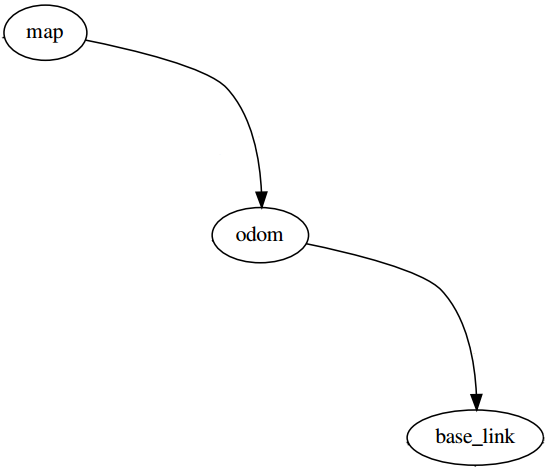
\includegraphics[width=0.5\textwidth]{frames.png}
       \end{figure}

    \end{frame}
    % -------------
    \subsection{Motion Model $g \left( u_t , \mu_{t}  \right)$ }
    \begin{frame}
        \justifying
        \frametitle{Motion Model $g \left( u_t , \mu_{t}  \right)$}
        The state vector $\mu$ (without markers \footnote{\tiny{Complete $\mu$ should be: $\begin{bmatrix} x & y & z & \psi & x_{1} & y_{1} & z_{1} & \psi_{1} & \dots & x_{j} & y_{j} & z_{j} & \psi_{j}\end{bmatrix}$\\ % hack to make the footnote visible
        }}) is: \\
        \begin{block}{}
            \centering
            $\mu = \begin{bmatrix} x^w & y^w & z^w & \psi \end{bmatrix}^T$
        \end{block}
        \begin{itemize}
            \item{$x^w \hspace{3pt} y^w \hspace{3pt} z^w $ represent the position of the drone in the map reference frame}
            \item{$\psi $ represents the drone's orientation in the map reference frame}
        \end{itemize}

    \end{frame}

    \begin{frame}
        \justifying

        The control vector \textit{u} is: \\
        \begin{block}{}
            \centering
            $u = \begin{bmatrix} v_x^b & v_y^b & v_z^b & \omega_x^b & \omega_y^b & \omega_z^b & \phi^b & \theta^b & \psi^b \end{bmatrix}^T$
        \end{block}
        \begin{itemize}
            \item{$v_x^b \hspace{3pt} v_y^b \hspace{3pt} v_z^b $ represent the linear velocity in the odometry (\textit{odom}) reference frame}
            \item{$\omega_x^b \hspace{3pt} \omega_y^b \hspace{3pt} \omega_z^b $ represents the angular velocity in the odometry reference frame}
            \item{$\phi^b \hspace{3pt} \theta^b \hspace{3pt} \psi^b $ represents pose of the drone as roll, pitch and yaw in the odometry reference frame}
        \end{itemize}

    \end{frame}

    \begin{frame}
        \justifying
        Since the control vector elements are in the \textit{odom} reference frame, we need to transform this into the \textit{map} reference so to store the drone's pose with respect to the world. \\[10pt]

        The motion model is then:
        \begin{block}{Position and orientation update}
            \begin{align*}
            \begin{bmatrix} \hat\mu_{r,x} \\ \hat\mu_{r,y} \\ \hat\mu_{r,z} \end{bmatrix} &= \begin{bmatrix} \mu_{r, x} \\ \mu_{r, y} \\ \mu_{r, z} \end{bmatrix}_t + \Delta t * \textbf{T} * \begin{bmatrix}
                u_{v_x} \\ u_{v_y} \\ u_{v_z}
            \end{bmatrix}
            \\
            \hat\mu_{r,\psi} &= \mu_{r,\psi} + \Delta t * u_{\omega_z}
            \end{align*}
        \end{block}

        \fontsize{9pt}{2pt}\begin{block}{Homogeneous transformation matrix (\textbf{T})}
            \centering
            $\begin{bmatrix}
            \cos{\psi}\cos{\theta} & \cos{\psi}\sin{\theta}\sin{\phi} - \sin{\psi}\cos{\phi} & \cos{\psi}\sin{\theta}\cos{\phi} + \sin{\psi}\sin{\phi} & 0\\
            \sin{\psi}\cos{\theta} & \sin{\psi}\sin{\theta}\sin{\phi} + \cos{\psi}\cos{\phi} & \sin{\psi}\sin{\theta}\cos{\phi} - \cos{\psi}\cos{\phi} & 0 \\
            -\sin{\theta} & \cos{\theta}\sin{\phi} & \cos{\theta}\cos{\phi} & 0 \\
            0 & 0 & 0 & 1
            \end{bmatrix}
            $
            \tiny{being $\phi$, $\theta$, $\psi$, roll, pitch, yaw respectively.}
        \end{block}

    \end{frame}

     % -------------
    \subsection{Observation Model $h \left( \hat\mu \right)$ }
    \begin{frame}
        \justifying
        \frametitle{Observation Model $h \left( \hat\mu \right)$}

        \begin{block}{Pole j}
            \begin{align*}
            \begin{bmatrix}
            p_{j, x}^b \\
            p_{j, y}^b \\
            p_{j, z}^b
            \end{bmatrix} &= \textbf{T}^{-1} \begin{bmatrix}
            p_{j, x}^w \\
            p_{j, y}^w \\
            p_{j, z}^w
            \end{bmatrix} \\
            p_{j,\rho}^b &= \sqrt{ p_{j, x^b}^2 + p_{j, y^b}^2 } \\
            p_{j, \alpha}^b &= \atantwo\left(p_{j, y}^b, p_{j, x}^b\right) \\
            p_{j, \beta}^b &= \atantwo\left(p_{j, z}^b, p_{j,\rho}^b\right)
            \end{align*}
            \tiny{being T the transformation matrix, where $T_{0; 3} = \mu_{x}$, $T_{1; 3} = \mu_{y}$ and $T_{2; 3} = \mu_{z}$ and $p_{j, z}^b$ represents the z value of the $j^{th}$-pole's tip}
        \end{block}
    \end{frame}

    \begin{frame}
        \begin{block}{Marker j}
            The drone has a camera looking downwards, and every time it sees a marker, a message is broadcasted with the marker's pose in the \textit{camera} frame. In order to estimate the marker's position and orientation, we move the pose in the \textit{camera} reference frame to the \textit{world} reference frame.
            \begin{align*}
                T_{m_j}^c &= (T_r^w * T_c^r)^{-1} * T_{m_j}^w
            \end{align*}
            Where $T_{m_j}^w$ is the marker's homogeneous transformation w.r.t the world reference frame, $T_r^w$ is the homogeneous transformation of the drone w.r.t the world reference frame, $T_c^r$ is the homogeneous transformation of the camera w.r.t the drone reference frame, and finally, $T_{m_j}^c$ is the marker's homogeneous transformation of the marker in the camera reference frame.
        \end{block}
    \end{frame}

    \begin{frame}
        \begin{block}{Marker j}
            From this homogeneous transformation matrix, we can extract the marker's position in the camera reference frame:
            \begin{align*}
                \begin{bmatrix} x_{m_j}^c \\ y_{m_j}^c \\ z_{m_j}^c \end{bmatrix} &= \begin{bmatrix} T_{m_j}^c(0;3) \\ T_{m_j}^c(1;3) \\ T_{m_j}^c(2;3) \end{bmatrix}
            \end{align*}
            We can also extract the marker's rotation in the camera reference frame:
            \begin{align*}
                \phi_{m_j}^c &= \atantwo\left(T_{m_j}^c(2;1), T_{m_j}^c(2;2)\right) \\
                \theta_{m_j}^c &= \atantwo\left(-T_{m_j}^c(2;0), \sqrt{T_{m_j}^c(2;1)^2 + T_{m_j}^c(2;2)^2}\right) \\
                \psi_{m_j}^c &= \atantwo\left(T_{m_j}^c(1;0), T_{m_j}^c(0;0)\right)
            \end{align*}
        \end{block}
    \end{frame}

% -------------
    \subsection{Inverse Observation Model $h^{-1} \left( \hat\mu \right)$}
    \begin{frame}
        \justifying
        \frametitle{Inverse Observation Model $h^{-1} \left( \hat\mu \right)$}
        \begin{block}{Marker j}
            The inverse observation model is used to add newly observed markers to the state vector. We obtain the marker pose w.r.t the camera reference frame, and we transform this to the map reference frame in the following way:
            \begin{align*}
            T_{m_j}^w &= T_r^w * T_c^r * T_{m_j}^c
            \end{align*}
            From $T_{m_j}^w$ we can extract the position w.r.t the world reference frame and the orientation w.r.t the world reference frame in the same way as in the observation model for markers.

        \end{block}
    \end{frame}

%    \begin{frame}
%       \begin{block}{Marker j}
%           From this homogeneous transformation matrix, we can extract the marker's position in the world reference frame:
%           \begin{align*}
%           \begin{bmatrix} x_{m_j}^w \\ y_{m_j}^w \\ z_{m_j}^w \end{bmatrix} &= \begin{bmatrix} T_{m_j}^w(0;3) \\ T_{m_j}^w(1;3) \\ T_{m_j}^w(2;3) \end{bmatrix}
%           \end{align*}
%           We can also extract the marker's rotation in the world reference frame:
%           \begin{align*}
%           \phi_{m_j}^w &= \atantwo\left(T_{m_j}^w(2;1), T_{m_j}^w(2;2)\right) \\
%           \theta_{m_j}^w &= \atantwo\left(-T_{m_j}^w(2;0), \sqrt{T_{m_j}^w(2;1)^2 + T_{m_j}^w(2;2)^2}\right) \\
%           \psi_{m_j}^w &= \atantwo\left(T_{m_j}^w(1;0), T_{m_j}^w(0;0)\right)
%           \end{align*}
%       \end{block}
%    \end{frame}

    % -----------------
    \section{Software Architecture}
    \subsection{Architecture overview}
    \begin{frame}
        \justifying
        \frametitle{Architecture overview}

        \begin{figure}
            \centering
            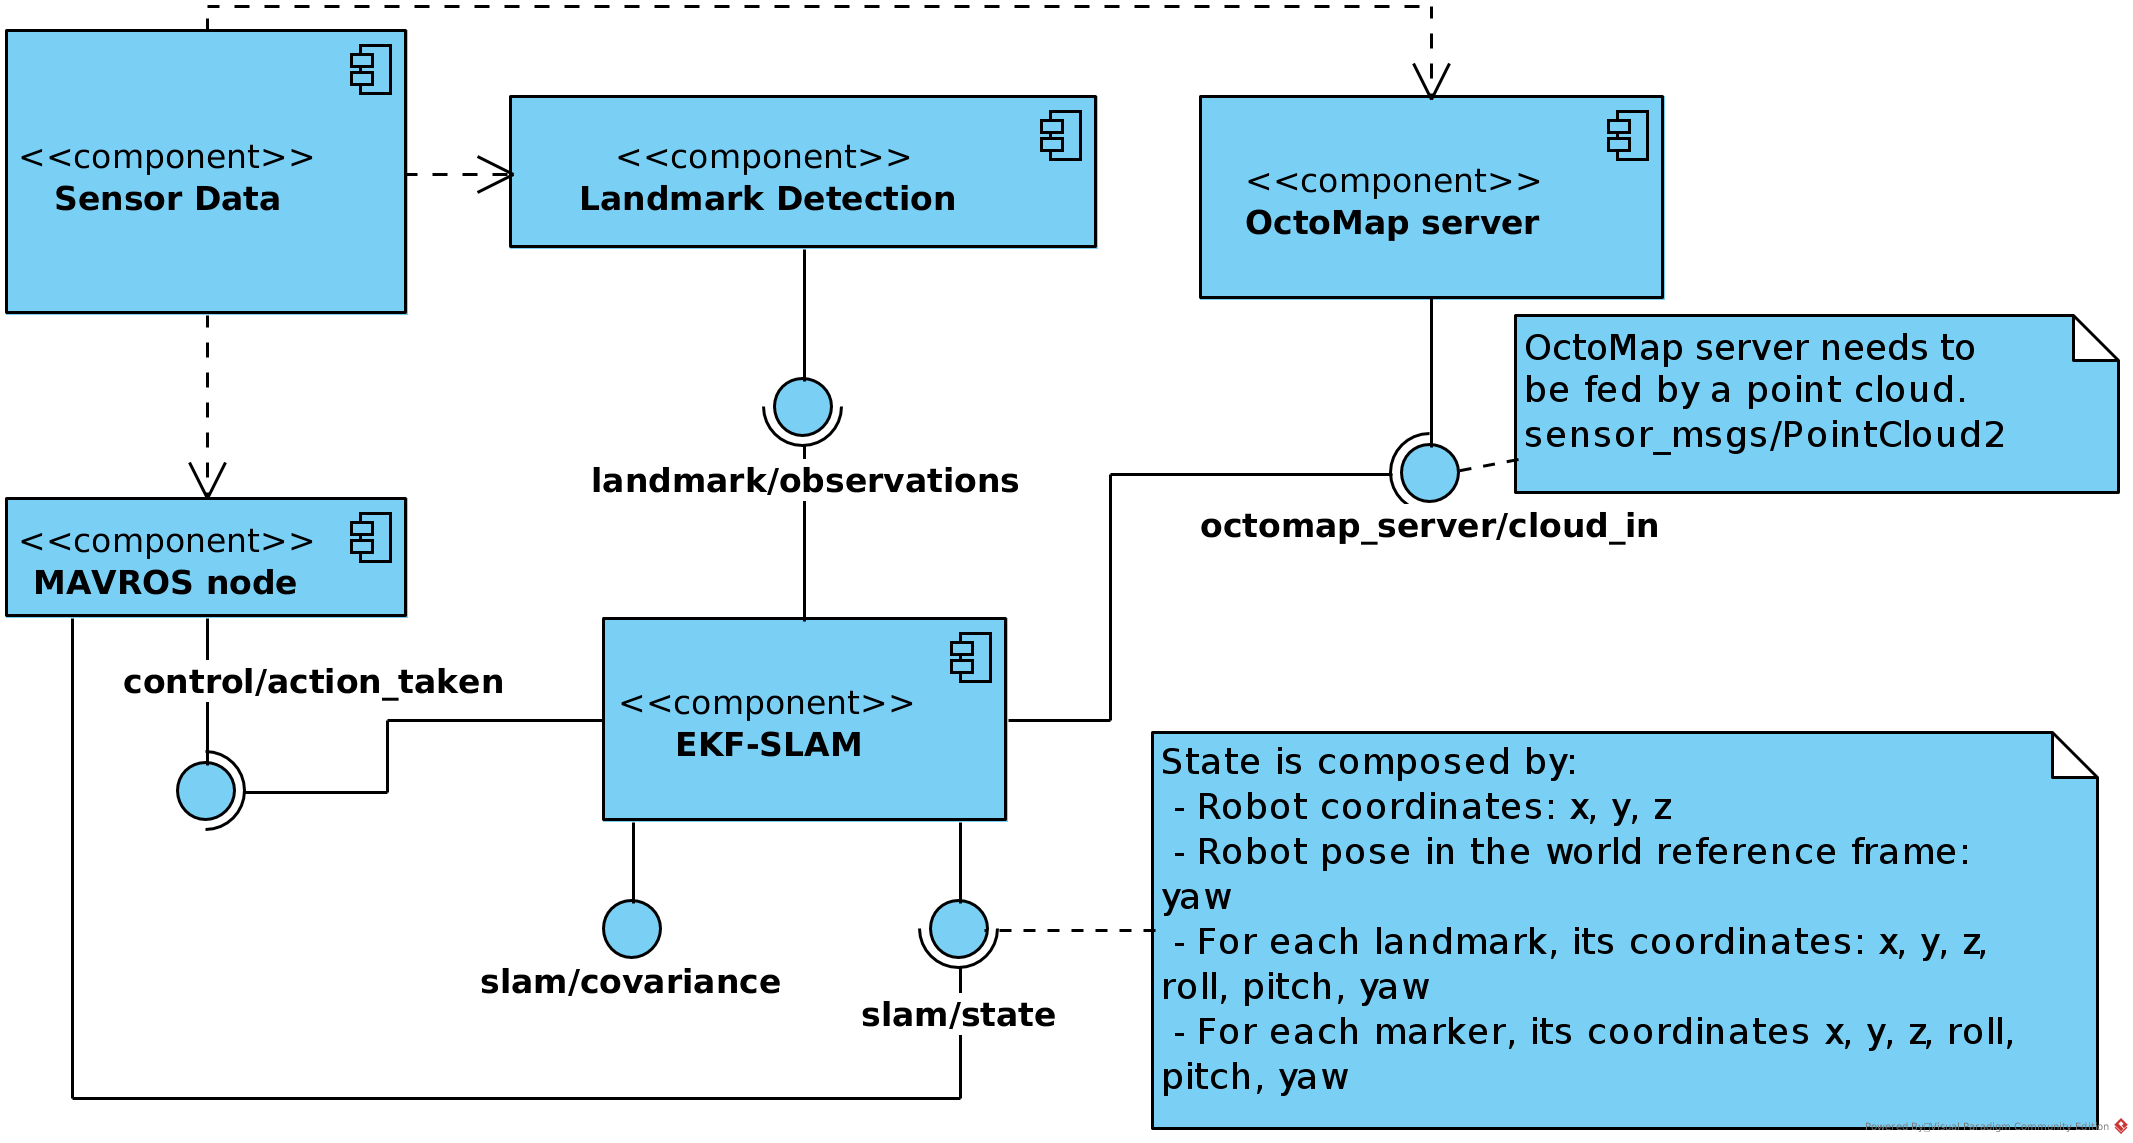
\includegraphics[width=\textwidth]{components.png}
        \end{figure}


    \end{frame}

    \begin{frame}
        The system's architecture has been done using ROS framework
        \begin{itemize}
            \item There is a ROS node which is responsible of detecting the landmarks and publishing its coordinates relative to the drone.
            \item Also, there is a control node, which is responsible of taking the control actions needed to drive the drone to the desired point.
            \begin{itemize}
                \item This node publishes the actions taken as pose increments
            \end{itemize}
            \item The EKF-SLAM node is responsible of update the state of the robot and keep track of the observed landmarks.
            \begin{itemize}
                \item It publishes the covariance matrix and the state vector at each time step
            \end{itemize}
            \item Finally, there is the OctoMap server, which should be fed with a point cloud
        \end{itemize}
    \end{frame}

    \subsection{Activity flow}
    \begin{frame}
        \justifying
        \frametitle{Activity flow}

        \begin{columns}
            \begin{column}{0.5\textwidth}
                \begin{figure}
                    \centering
                    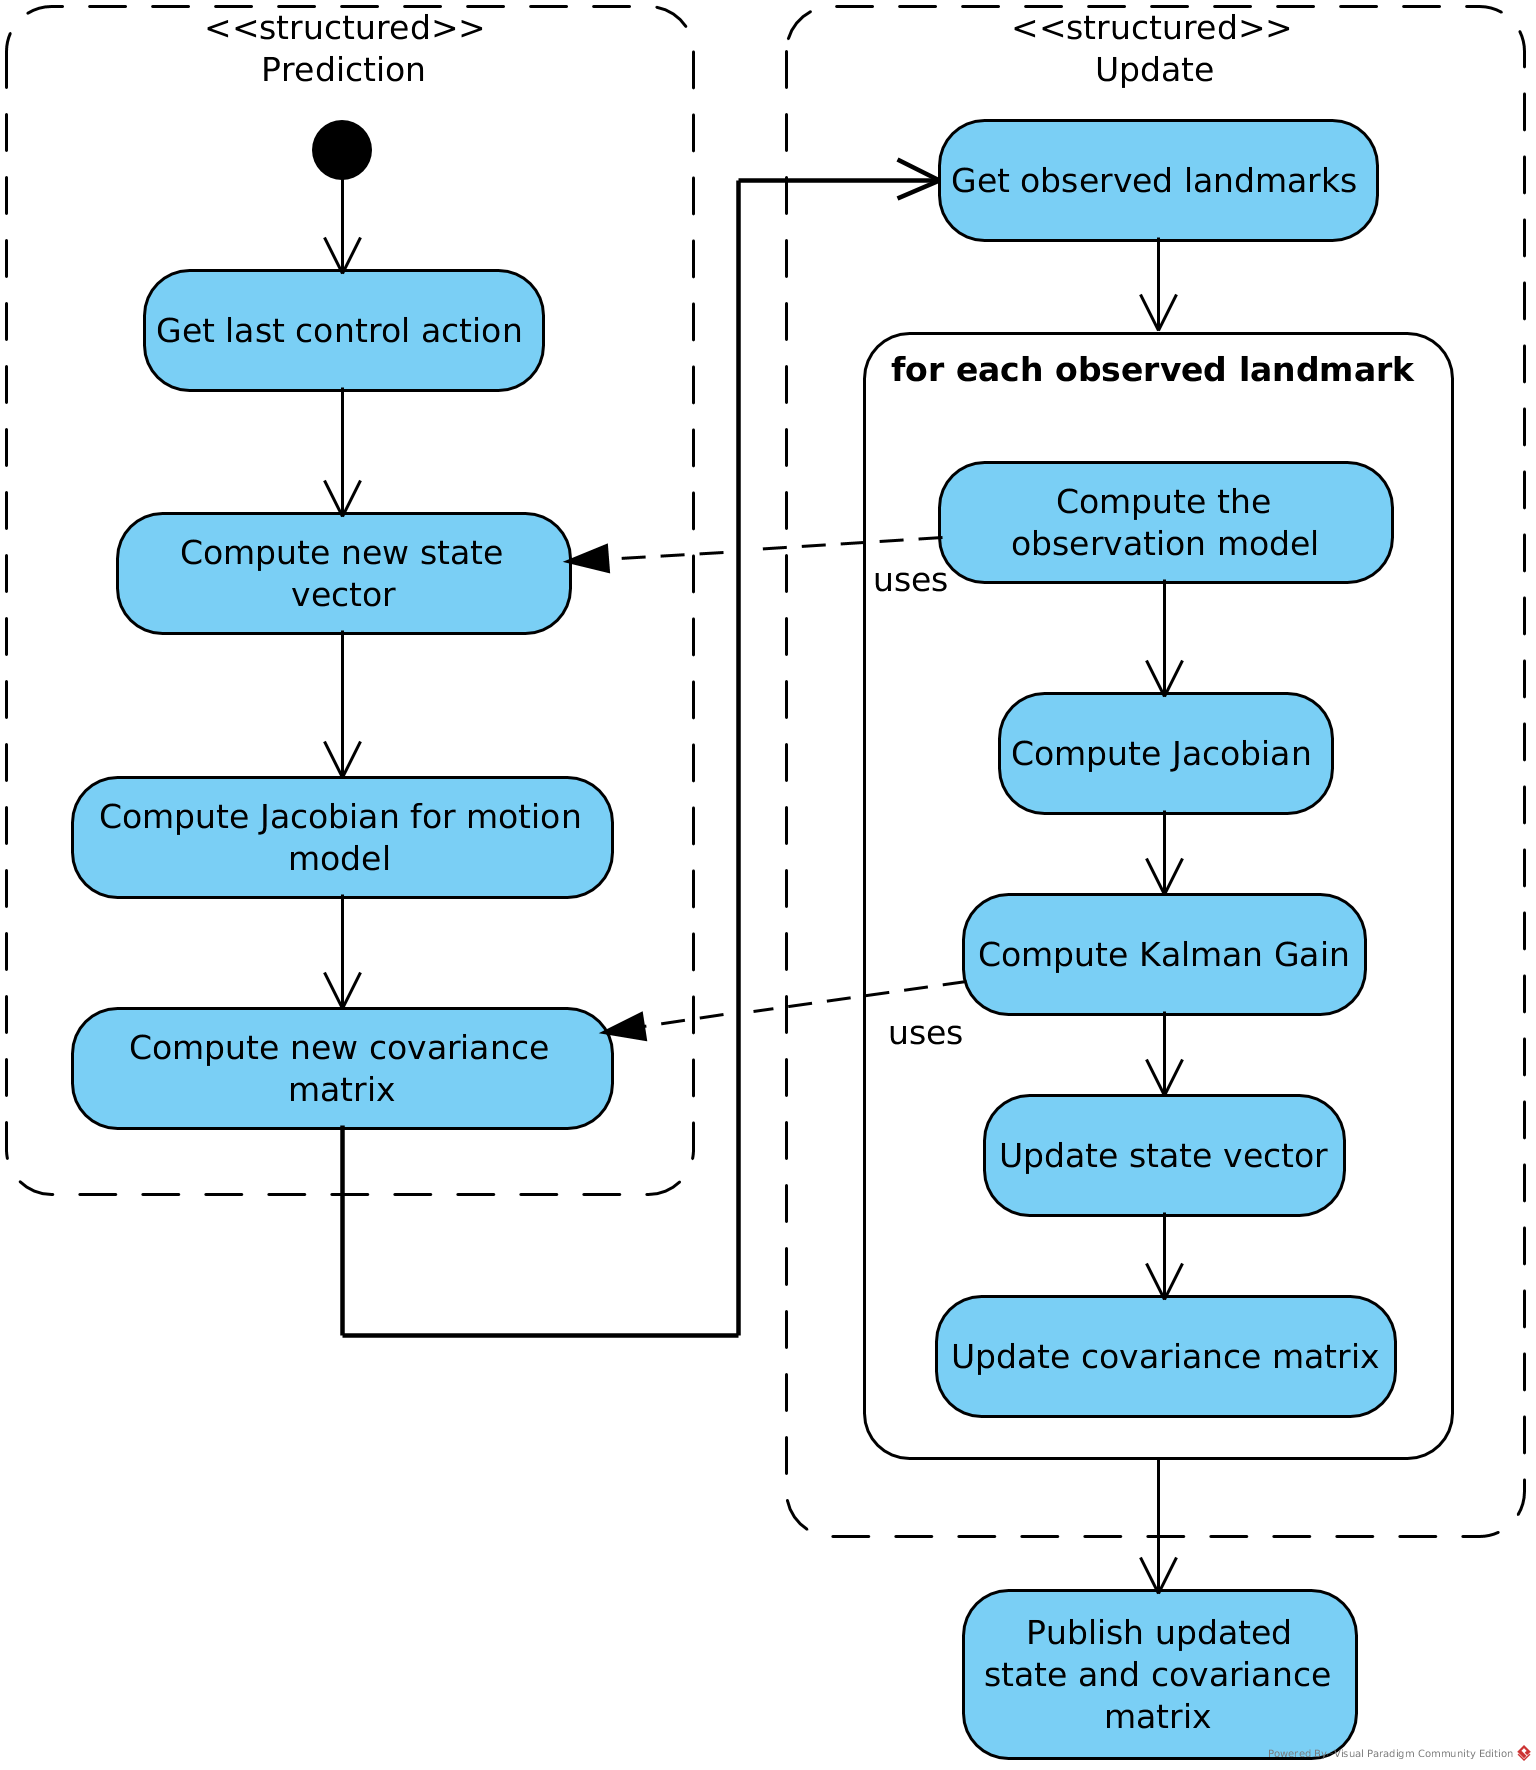
\includegraphics[width=\textwidth]{activity.png}
                \end{figure}
            \end{column}
            \begin{column}{0.5\textwidth}
                In the following activity diagram it can be seen the computation of the state vector and the covariance matrix. \\[10pt]

                Also, at the end of the update stage, it publishes the final state vector.
            \end{column}
        \end{columns}


    \end{frame}

    % -----------------
    \section{Conclusion}
    \begin{frame}
        \justifying
        \frametitle{Conclusion}
        Considering that several things need to be defined, it seems that an EKF-SLAM should not be complicated to implement. \\[10pt]

        As stated by \cite{Bailey1}: \\

        \blockquote{Implementing SLAM in 3-D is, in principle, a straightforward extension of the 2-D case. However, it involves significant added complexity due to the more general vehicle motion model and, most importantly, greatly increased sensing and feature modeling complexity}

        Finally, I have found several EKF-SLAM implementations, being the MRPT (\citet{6dofekfslamBlanco}) implementation the most general one. Moreover, it has a wrapper for ROS called mrpt\_navigation (\citet{blancoMRPT}), but it is not clear whether it accepts 3D maps

    \end{frame}

    % -----------------
    \section{References}
    \begin{frame}[allowframebreaks]
        \frametitle{References}

        \nocite{2,3,4,5,6,7,8,9,10,11,12,13,14}
        \bibliography{references.bib}

    \end{frame}





\end{document}
